% to submit via https://www.easychair.org/account/signin.cgi?conf=europar2013
% max 12 pages
\documentclass{llncs}
%
\usepackage{listings}
\usepackage{url}
\usepackage{todo}
\newcommand\see{\emph{cf.\ }}

\usepackage{tikz}
\usetikzlibrary{positioning}
\usetikzlibrary{shadows}
\usetikzlibrary{arrows}


\lstset{language=python}

\begin{document}
%
\title{Pythran: Bringing OpenMP to a Python Subset}

\author{Serge Guelton\inst{1,2} \and Pierrick Brunet\inst{2}}

\institute{
    {\'E}cole Normale Sup{\'e}rieure, Paris, France
    \and
    T{\'e}l{\'e}com Bretagne, Plouzan{\'e}, France
}

\maketitle

%
\begin{abstract}

    The Python language offers an interesting alternative as a scientific
    computing language thanks to the SciPy package. However, the lack of
    fine-grained parallelism support remains an important shortcoming. This
    paper proposes to add OpenMP directives to the Python language and shows
    that it is possible to turn a module written in a large Python subset
    enhanced with these directive into a native parallel module that runs as
    fast as its naive C equivalent. The approach is validated through the
    Pythran compiler.

\keywords{Python, OpenMP, C++, static compilation, scripting language}
\end{abstract}

%
\section{Introduction}

Since its birth in December 1989, the Python language~\cite{rossum97} has proved
to be useful in various domains, ranging from system administration to web
services, thanks to its dynamicity, expressiveness, rich ecosystem and
battery-included standard library. It is also getting widely used in scientific
computing~\cite{Oliphant2007}, mainly thanks to the SciPy~\cite{scipy} project
that adds Matlab-like functionalities to the language.

The prohibitive performance overhead of the language implied by its interpreted
and highly dynamic nature should prevent its usage as a language for high
performance computing. SciPy overcomes this issue through the usage of low-level
routines written in C or Fortran and encapsulated in Python through
\emph{native} modules. Moreover, its core data structure, the multi-dimensional
array~\cite{numpyarray2011}, was designed so that the underlying data are
available to both native modules and the Python interpreter without conversion
costs.

To make it easier for the user to write native functions, \emph{i.e.}\ without
having to write the glue code that turns Python object into native structures
back and forth, the SciPy package provides the \texttt{weave} module that makes
it possible to bundle C code snippet into Python code and compile then load them
at runtime.

This hybrid approach, based on a mix of interpreted and native code, is getting
wide spread in the Python landscape. Section~\ref{sec:python-parallel} studies
the existing approaches and shows a critical lack of parallelism support.
Section~\ref{sec:python-openmp} studies the validity of adding OpenMP directives
to the Python language in order to add fine-grain parallelism support to Python
in the context of a Python subset called Pythran. Static compilation of this
language into C++ and the underlying runtime is described in
Section~\ref{sec:python-static}. The Pythran compiler is benchmarked on several
scientific applications and compared to both interpreted and native code in
Section~\ref{sec:validation}.

%=========================================================
\section{Parallel Computations in Python}\label{sec:python-parallel}
%=========================================================

In the many cores area, turning to parallelism to balance the performance
limitations of scripting languages, as described in~\cite{choy05} in the context
of the MATLAB language, or in~\cite{mals07} in the context of the R language,
seems legitimate. In the context of Python, most approaches have
focused on fork-based parallelism.

\subsection{Python and Parallelism}

Parallel computations are supported by the Python standard library through the
\texttt{multiprocessing} module. It spawns several interpreters that can
communicate through IPC, using Python built-in object serialization. This
approach is only viable for computation intensive application, but the
communication and synchronization overheads are much greater than a light-weight
processes approach.

Although the standard \texttt{threading} module makes it possible to start
several light-weight threads within the same interpreter, this approach is not
relevant for HPC, because of a specificity of CPython, the \emph{Global
Interpreter Lock}~\cite{gil2012}~\footnote{Other Python interpreters, such as
IronPython or Jython, do not have a GIL.} This lock ensures only one thread is
active at a time in the interpreter. While it make it possible to have
cooperative thread, say for a GUI, it does not take advantage of multiple cores.
However, there are two notable exceptions: the GIL is released on I/O, and the
GIl does not prevent the use of threads inside native modules, where the user
has full control.

As a consequence, Python developers need to write multi-threaded native
modules in order to fully benefit from multiple cores. This lead to a kind of
computations referred as hybrid computations.

%There have been several approaches to replace the GIL by Transactional
%Memories~\cite{Riley2006,Tabba2010} but none of them made there way to the
%mainstream interpreters.


\subsection{Hybrid Computations}

In the context of interpreted language, an hybrid computation is defined
in~\cite{dongara2007} as a computation where part of the code is interpreted,
and part of the code is executed natively.

It is now common for scripting language to have C bindings. To take advantage of
compiled code, and to overcome the GIL limitations, Python developers must write
parallel C/C++ functions and the associated boilerplate based on the Python C
API~\cite{pythoncapi}. Tools have been developed to relieve the user from
writing the encapsulating code, notably Swig~\cite{swig2003} that relies on an
enhanced interface specification, or
\texttt{boost::python}~\cite{boostpython2007} that relies on C++ facilities to
guide translation.

An opposite approach consists in using the host language ---herein Python---
to describe both parts of the system, and to let an automated tool perform the
translation to native code of a part of the application, generally the
computation-intensive one where parallelism has been expressed in some ways.
Thus, developers not familiar with lower level language or not eager to invest
the additional development time can still benefit from a fair performance boost.
This approach has been subject to many studies that can be classified based on
their backward-compatibity with the host language.

\subsubsection{Backward-Incompatible Approaches}

A constraining (from the performance point of view) aspect of the Python
language is its type system. It has several consequences, among which the fact
that each method call is resolved dynamically, including a simple add
operation! It comes at no surprise that many approaches extend the Python
language to add a static typing overlay. Likewise, there is only two types of
integers (64bits integers and multi-precision integers) and one type of floating
point type (double-precision floats) in Python, while using a type with the
appropriate size may lead to significant performance boost.

Cython~\cite{cython2010} is such a Python dialect. It extends the syntax with
typing informations, calls to native functions from third party libraries, and a
limited set of parallelism constructs, among which the possibility to define
parallel loops, but no task parallelism. Plw~\cite{dongara2007} proposes a
similar approach that mixes Python with C, using raw strings to hold the C code
and the parallel directives, that are limited to parallel for loops.  The
numba~\footnote{\emph{cf}.\ \texttt{https://github.com/numba/numba}} compiler
uses additional type information to generate sequential LLVM bytecode.  PyCUDA
and PyOpenCL~\cite{klockner2012} also mixes python with kernels embeded as raw
strings to target accelerators.

The core issue of these approaches is that they imply to modify, in a more or
less trivial way, the original code. They require to invest in a new language,
and the long-term preservation of this investment is not ensured.

\subsubsection{Backward-Compatible Approaches}

Most backward-compatible approaches also require to modify the input program,
but they do not extend the Python language, rather restrict it. As a
consequence, they remain compatible with the original language and do not suffer
from the drawbacks of the previous approach.

Copperhead~\cite{shedskin2006} is a functional, data parallel language embedded in
Python. It uses n-uplets, Numpy arrays and lists as its core data structure and
prohibits usage of many control-flow operators such as loops, enforcing the use
of the \texttt{map}, \texttt{filter} or \texttt{reduce} intrinsics to exhibit
parallelism. In returns, it can be efficiently compiled to either CUDA or C++
with calls to the Thrust~\footnote{\emph{cf}.\
\texttt{http://thrust.github.com/}} library. Python decorators are used to
identify hot-spots that are dynamically compiled to native code.

Tools such as PyPy~\cite{pypy2009}, a Python interpreter with a tracing JIT, or
Shedskin~\cite{shedskin2006}, a Python to C++ compiler also are viable way to
turn regular Python codes into optimized ones, but they do not offer support for
fine-grained parallelism beyond what the standard library
proposes.
%~\footnote{Shedskin is compatible with several Python modules that
%provide coarse-grained, fork-based parallelism.}

This article proposes to combine OpenMP~\cite{openmp3.1} parallel annotations
with a Python subset called Pythran to bring fine-grain parallelism to Python
while being backward compatible with both the Python language, and the
sequential algorithm. It means that:
\begin{enumerate}
    \item Any Pythran code can be run (sequentially), with no module dependency or code change,
        by any Python interpreter.
    \item Parallelism is explicit and incrementally added to the original code
        through directives.
\end{enumerate}

%=========================================================
\section{OpenMP Semantic Adaptations}\label{sec:python-openmp}
%=========================================================

OpenMP is a standard API for parallel programming for Fortran, C and C++. It
consists in a set of parallelizing directives and a few runtime library calls.
If OpenMP is not activated, the directives are ignored, thus enabling
incremental parallelization of the original source code while keeping the
original code structure.

The languages targeted by OpenMP are statically compiled. This section studies
the semantic adaptation required to use the same API for a scripting language
such as Python.

\subsection{Directives}

OpenMP directives are held by C/C++ pragma, or by Fortran comments. Most of them apply
on structured blocks, represented by an instruction in C/C++ and delimited by
comment in Fortran. A few directives (e.g.\ \texttt{threadprivate}) are not
attached to a specific instruction.

While Pythran does have a decorator mechanism~\footnote{\see PEP 319,
\url{http://www.python.org/dev/peps/pep-0318/} for a more detail explanation fo
Python decorators.}, it only applies to functions, methods and classes and does
not make it possible to attach decorations to random instructions.
PLW~\cite{dongara2007} suggests to use string instructions to hold such
decorations. As Python does not have anonymous block~\footnote{\see PEP340,
    \url{http://www.python.org/dev/peps/pep-0340/} for a discussion concerning
anonymous block support in Python.}, one has to create a dummy \texttt{if 1:}
instruction to apply an annotation to a whole block. Alternatively, the syntax
\texttt{if 'my annotation':} is also supported.
Listing~\ref{lst:instruction-annotation} shows how to annotate a parallel loop
with reduction this way.

\begin{figure}
    \begin{lstlisting}[label={lst:instruction-annotation}, caption={Parallel
    loop with reduction annotated with OpenMP directive.}]
'omp parallel for reduction(+:r)'
for auto in my_container:
  r += x
  \end{lstlisting}
\end{figure}

Many OpenMP annotations are parametrized by clauses that list variables,
specifying their behavior with respect to parallel regions, e.g.\
\texttt{private}, \texttt{shared}, \texttt{copyin}. They can only refer to
variables that have already been declared. However, there is no variable
declaration in Python, and all variables assigned in a function have the
function scope. Consequently, all variables referred to in a function are to be
considered when building such variable lists: there is no concept of variable
local to a block. Using the \texttt{default(none)} clause is possible to ensure
that no variable gets forgotten when building such lists, as a compile-time
error is raised if a variable is referred in a block but not in the associated
parallel region.

The \texttt{reduction(\emph{operator}: \emph{list})} is used to handle data
dependencies when performing a parallel reduction. The supported operator
depends on the input and backend language: Python has \texttt{min}/\texttt{max} operators but
C/C++ have not. Python does not have \texttt{\&\&} or \texttt{||}
operators~\footnote{Although similar, the \texttt{and} and \texttt{or} keywords
have a special meaning in Python.} while C/C++ have.

\subsubsection{Parallel For and Iterators}

The core directive to handle data parallelism is the \texttt{for} directive that
distribute the iteration space of the associated loop among the existing
threads. To be compatible with OpenMP, the loop iteration space must be
described by a random access iterator with a total order, i.e.\ it is possible
to increase the iterator by any integer and to decide which iterator is the
greatest among two. The integer used as loop indices in Fortran and C satisfy
this conditions, so do C++ iterators with the \texttt{random\_access\_tag}
trait. But a Python iterator only advance by a step of one until it is
exhausted, in which case it raises an exception. They only have forward iterator
behavior.

The extension of Python iterator to random access iterators is direct for the
standard containers: \texttt{list}~\footnote{Python \texttt{list}s behave as C++
\texttt{vector}s.}, \texttt{set} or \texttt{dict}.

Python also generalizes the concept of iterators through generators, which also
behave like forward iterators. The simplest one, \texttt{xrange(\emph{start},
\emph{stop}, \emph{step})}, successively yields value starting from
\texttt\emph{start} to \texttt\emph{stop} by a step of \texttt\emph{step}. It is
easily extended to support random access, but it generally does not make
sense to use a generator as a loop iterator, as the relation between two
random states of the iterator may be of an arbitrary complexity.

A particular class of generator behaves like adaptor, in the sense that they
apply a particular expression on each value of the iterator. It is the case of
the \texttt{enumerate} builtin that yields each element of the enumerated
iterator associated with its index. Generator expressions such as \texttt{(x*x
for x in l)} have the same behavior. These generators are random iterators only
if their input iterator is a random iterator itself.

Finally, if the iterator yields a tuple, it is possible to unpack it inside the
\texttt{for} construct, as shown in Listing~\ref{lst:complex-omp-for}. In that case
all the unpacked variables are considered as iterators, especially with respect
to default privatization rules. In the given example, \texttt{i} and \texttt{v}
are private, and the parallel iteration is valid because the input of
\texttt{enumerate} is a list, which allows random access iteration.

\begin{figure}
    \begin{lstlisting}[label={lst:complex-omp-for}, caption={Parallel
    loop with tuple unpacking.}]
'omp parallel for'
for i, v in enumerate([2, 3, 5, 7, 11]):
  print i, ':', v
  \end{lstlisting}
\end{figure}

\subsection{Runtime Library}

The OpenMP runtime library makes it possible to retrieve the active thread id,
whether dynamic scheduling is enabled and so on. All the functions are declared
in the \texttt{<omp.h>} header, and have a default behavior when OpenMP is not
activated.

Providing a biding to these library in the Python does not raise
particular problems, as the signature of these functions only involves passing
integers as parameters or return values, except for the mutex manipulation. In
that case an opaque type is used to represent the native type.

The \texttt{\_OPENMP} macro definition is always provided when OpenMP is
activated, and can be used for portability with system where OpenMP is not
available. Python does not have a preprocessor, but it is possible to catch the
import exception if the \texttt{omp} module is not found.

\subsection{Validation}

A validation suite for OpenMP has been proposed in~\cite{wang2012} for C and
Fortran. We have ported it to Python, and we also extended it to validate the
corner cases specific to Python described in this section. An example of such
test case is given in Listing~\ref{lst:openmp-validation}.

\begin{figure}
    \begin{lstlisting}[label={lst:openmp-validation},caption={Example of Python
    OpenMP validation test case.}]
def omp_parallel_for_if():
  import omp
  using = num_threads = 0
  sum = sum2 = 0
  LOOPCOUNT = 1000
  'omp parallel for private(i) if(using == 1)'
  for i in range(LOOPCOUNT + 1):
    num_threads = omp.get_num_threads()
    sum += i
  known_sum = (LOOPCOUNT * (LOOPCOUNT + 1)) / 2
  return known_sum == sum and num_threads == 1
    \end{lstlisting}
\end{figure}

We have used the Pythran tool described in the following section to turn each
Python test function into a C++ function with the same directives and runtime
calls. Apart from the \texttt{threadprivate} directive and the
\texttt{collapse(\emph{n})} clause, all tests were successful.
\texttt{threadprivate} directives were held by global variables not supported in
Pythran yet~; and the C++ code generated by Pythran does not preserve the perfect
loop nesting required by the \texttt{collapse} clause.

%=========================================================
\section{Static Translation of Python Programs}\label{sec:python-static}
%=========================================================

Pythran is subset of Python focused on scientific computing. It is implicitly
statically typed and support most Python constructs except those that involve
introspection (e.g.\ \texttt{getattr}) or runtime compilation (e.g.\
\texttt{eval}). A few standard module are supported in addition to the core
language (e.g.\ \texttt{math}, \texttt{random}). The \texttt{numpy} module is
partially supported. The associated compiler turns Pythran code, eventually
annotated with OpenMP and exported function type annotation, into C++ code. Its
processing is summarized in Figure~\ref{fig:pythran-compiler}. The purpose of
this section is not to dig into the internal of the compiler, but rather to
focus on the impact of the parallelism layer, especially on the runtime library,
\texttt{pythonic}.

\begin{figure}

\centering
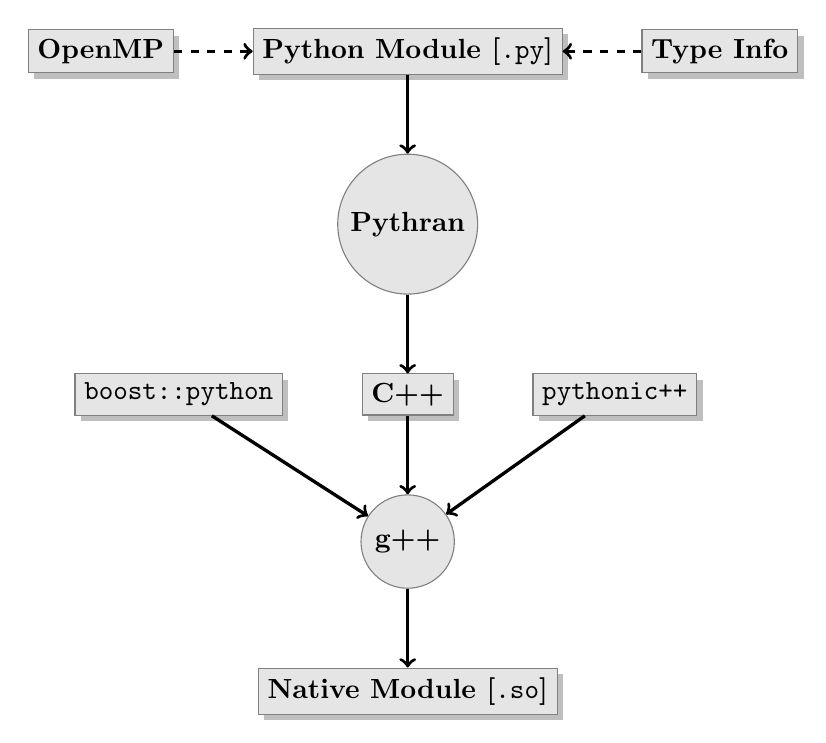
\begin{tikzpicture}[
file/.style={draw=black!50,fill=black!10,rectangle, drop shadow, align=center},
    tool/.style={draw=black!50,fill=black!10,circle, align=center}]
    \node[file] (python) {\textbf{Python Module [\texttt{.py}]}};
\node[file] (annotation)	   [right=of python] {\textbf{Type Info}};
\node[file] (omp)	   [left=of python] {\textbf{OpenMP}};
\node[tool] (pythran) [below=of python] {\textbf{Pythran}};
\node[file] (cxx) [below=of pythran] {\textbf{C++}};
\node[file] (boost) [left=of cxx] {\textbf{\texttt{boost::python}}};
\node[file] (pythonic) [right=of cxx] {\textbf{\texttt{pythonic++}}};
\node[tool] (gxx) [below=of cxx] {\textbf{g++}};
\node[file] (so) [below=of gxx] {\textbf{Native Module [\texttt{.so}]}};

\draw[very thick, ->] (python) -- (pythran);
\draw[very thick,dashed, ->] (annotation) -- (python);
\draw[very thick,dashed, ->] (omp) -- (python);
\draw[very thick, ->] (pythran) -- (cxx);
\draw[very thick, ->] (cxx) -- (gxx);
\draw[very thick, ->] (boost) -- (gxx);
\draw[very thick, ->] (pythonic) -- (gxx);
\draw[very thick, ->] (gxx) -- (so);
\end{tikzpicture}
\caption{Pythran compiler workflow.}
\label{fig:pythran-compiler}
\end{figure}

\subsection{Runtime Support}

The standard library of C++11, unlike its C++03 version, is thread-safe. Pythran
runtime is based on the STL and provides the same guaranty, so that the data
dependences in the original code remains explicit.

A critical point when designing the pythonic runtime was memory management, the
very same aspect that lead to the use of a GIL in CPython. Pythran handles the
problem by refusing recursive types, which makes it possible to solely rely on
reference counting for memory management. It can be implemented through the
thread-safe shared pointer mechanism provided in C++11 standard library.

Using shared references simplifies memory management, but the counterpart is an
extra atomic operation for each copy. It limits parallelism, so reducing the
number of copies remains an important goal. The move semantic introduced in
C++11 avoids a few copies when working on temporary objects, but argument
passing may be a trouble. To avoid a reference increment, one can use pass
parameters by reference. Using an interprocedural memory effect analysis, Pythran
determines for each argument whether it must be passed using reference or const
reference to prevent this extra cost.

\subsection{Directive Oblivious Translation}

During Python to C++ translation, Pythran adopts a blind strategy: it does not
understand the semantic of the annotations. Instead, it just split each
annotation into a context-sensitive part ---the variable names--- and a
context-insensitive part ---the clauses---, and attach them to the proper
instruction in the AST. It then ensures a bijective translation between Python
instruction and generated C++ instruction so that the OpenMP directive is
regenerated on the proper instruction. The same approach is used at the
expression level, to be compatible with the \texttt{if} clause.

\subsection{Transfer Costs}

When passing containers from Python to C back and forth, a copy of the whole
data is made to turn the type agnostic, non-contiguous Python data into dense
typed ones. This extra copy implies an extra cost that is not negligible: the
time taken to pass two lists of float from Python to C++ is only twice less than
the time taken to compute the dot product of the same lists directly in Python.
Following Amdahl's law, this transfer cost greatly hinders parallelization, and
is a well known issue.

The traditional solution is to use a native type that exposes a Python interface
and has a constant translation cost. Numpy's \texttt{ndarray} is a typical
implementation of this concept and is the keystone of the Scipy and Numpy
packages. Basically, a numpy \texttt{ndarray} is a raw C pointer that is exposed
at the Python level. As a tool for scientific computing, Pythran supports such a
structure.

%=========================================================
\section{Validation}\label{sec:validation}
%=========================================================

To validate the approach proposed in this paper, we first performed a simple
experiment. Starting from the C code of a small geomatics application, we
successively parallelized it with OpenMP, turned it into Python with a Pythran
compatible kernel and parallelized the Python version using the approach
described in this paper. We also measurer the SLOC for the two versions.
Table~\ref{tbl:hyantes} summarizes the results of the experimentation made on a
laptop with 4 non hyperthreaded cores using \texttt{-O2} compiler flag. It
non only emphasises the use of a high level language prototyping, but also shows
that it is possible to turn this prototype into reasonably efficient code
through Pythran. It is also possible to prototype the parallel version while
remaining at the Python level.

\begin{table}

    \centering
    \begin{tabular}{|l|l|l|l|}
        \hline
        Language & SLOC & wall time (s) [gcc] & wall time (s) [clang]\\
        \hline
        C       & 102   & 25 & 22 \\
        Python  & 30    & 676 & --\\
        Pythran & 30    & 38 &  22 \\
        Pythran+OMP    & 30    & 11 & no OpenMP support\\
        \hline
    \end{tabular}

    \caption{Comparison of several versions of the Hyantes prototype.}
    \label{tbl:hyantes}

\end{table}


We then compare Pythran with Cython. The approach share some similarities: they
both generate code written in a rather low level language, with OpenMP
directives. However, the inputs differ as Cython requires more typing
information that Pythran to generate efficient code, and Cython is not
backward-compatible with Python. They both translate explicit fine-grained
parallelism through code annotations or specific python constructs,
respectively.

Pythran exposes the full OpenMP interface to the user, thus enabling both data
and task parallelism, as described in Section~\ref{sec:python-openmp}. This is
not the case in Cython, where:

\begin{itemize}
    \item Only loops can be made parallel, through the use of a dedicated
        intrinsic \texttt{prange} as loop iterator. To use more advanced
        parallelism construction, one must rely on the possibility to write raw C
        code embedded in cython.~\todo{SG->PB: tu m'explique ce truc de C dans
        cython ?}

    \item Cython automatically infers reductions and variable privacy, giving
        less control to the end-user.

    \item As Cython allows the mix of Python and Cython code, the user is
        responsible from releasing the GIL.

    \item The code included in a parallel region interacts with the Python code
        in a restricted manner. For instance, it is impossible to use a function
        imported from a Python module, while it is still possible to use native
        C functions.
\end{itemize}

Listings~\ref{lst:cython-sample} and~\ref{lst:pythran-sample} illustrates the
difference between the two approaches. It shows that while being more integrated
in Python, the Cython approach is more verbose.

\begin{figure}[ht]

    \begin{lstlisting}[label={lst:cython-sample}, caption={Cython Impelmentation
    of a Parallel Reduction.}]
import math
cimport cython
from cython.parallel import parallel, prange
from libc.math cimport sqrt
def sum_sqrt():
    cdef float r = 0
    cdef int i
    with nogil, parallel():
        for i in prange(10000000):
            r += sqrt(i)
    return r
\end{lstlisting}
\end{figure}
%
\begin{figure}[ht]
    \begin{lstlisting}[label={lst:pythran-sample}, caption={Cython Impelmentation
    of a Parallel Reduction.}]
#pythran export sum_sqrt()
import math
def sum_sqrt():
    r = 0
    "omp parallel for private(i) reduction(+:r)"
    for i in xrange(10000000):
        r += math.sqrt(i)
    return r
    \end{lstlisting}
\end{figure}



The performance of the two approaches is illustrated in
Figure~\ref{fig:cython-pythran}.

\begin{figure}[ht]
    
\includegraphics[width=\textwidth]{cython}
    \caption{Comparison of Cython en Pythran generated code performance.}
    \label{fig:cython-pythran}
\end{figure}

The benchmarked codes are typical mathematical, image-processing or linear
algebra kernels. All these kernels have been written in Cython and Python
---compatible with Pythran--- and annotated through the mechanism of each
language to exhibit parallelism, then compiled into native code using GCC 4.1
and the \texttt{-O2 -fopenmp} flag. Their execution time when called from the
Python interpreter is measured through the \texttt{timeit} module. All results
are normalized to Cython sequential execution time.

This figure shows our inability to select proper benchmarking code, and to run
them on a real multiprocessor machine, but this is gonna change!~\todo{SG->PB:
c'est pour toi !}

All the source codes used for these benchmarks are availabe on the Pythran
reporsitory.~\footnote{\emph{cf}.\
\texttt{https://github.com/serge-sans-paille/pythran} on \texttt{europar2013}
branch.} 


%=========================================================
\section{Conclusion and Future Work}
%=========================================================

This paper studies the relevancy of adding OpenMP annotations to Python code. It
shows that providing minor semantic adaptations, these annotations are relevant
and makes it possible for Python code to benefit from multi-core performance
boost without worrying about the Global Interpreter Lock.

To achieve this goal, a translator from a subset of the Python language to C++
has been designed. This translator can turn regular Python modules
annotated with OpenMP directives and a few type annotations into native parallel
module. Both the input module and the generated one remain compatible with the
standard interpreter.

The approach is compared with Cython, an extension of the Python language used
to generate native module with an hybrid Python-C syntax that also provide means
to exhibits fine grained parallelism. Modules generated by Pythran outperform
modules generated by Cython for various kernels and both benefit from the
parallel boost.

Future works include the extension of the approach to OpenMP 4 and the
\texttt{target} clause that should make it possible to target MIC from Python.
There is also many vectorization possibility in Python, especially in the list
comprehension construction, that needs to be explored.

%=========================================================
\section*{Acknowledgments}
%=========================================================

This work has received fundings from the \texttt{Silkan} company and the French
ANR through the CARP project. The authors would like to thanks Adrien
\textsc{Merlini} and Alan \textsc{Raynaud} for their work on the C++ runtime.
Fabien \textsc{Dagnat} and Mehdi \textsc{Amini} also contributed to this paper
through their many valuable advices.

\bibliographystyle{splncs03}
\bibliography{biblio}

\end{document}
% vim:spell spelllang=en
% vim:tw=80
